\documentclass[11pt, a4paper]{article}
%\usepackage{proj1}
\usepackage{natbib}
\usepackage{fancyhdr}  
\usepackage{subcaption}
\usepackage{caption}
\usepackage{graphicx}
\linespread{1.25} 
\setlength{\parindent}{0cm}
\graphicspath{{Images/}}
\usepackage{hyperref}
\usepackage{amsmath}
\usepackage{amsfonts}
\usepackage{amssymb}
\usepackage{amsthm}
\usepackage{mathtools}
\usepackage{commath}

%\usepackage[sc,osf]{mathpazo}
\usepackage{subcaption}
\usepackage[a4paper, top=1in, left=1.0in, right=1.0in, bottom=1in, includehead, includefoot]{geometry} %Usually have top as 1in

\usepackage{listings}
\usepackage{color} %red, green, blue, yellow, cyan, magenta, black, white
\definecolor{mygreen}{RGB}{28,172,0} % color values Red, Green, Blue
\definecolor{mylilas}{RGB}{170,55,241}


\hypersetup{colorlinks,linkcolor={black},citecolor={blue},urlcolor={black}}
\usepackage{color}
\urlstyle{same}


\theoremstyle{definition}
\newtheorem{definition}{Definition}[section]

\title{Exact Solutions for the Full Problem \\with Force Control and with Flow Control}
\date{}
\newcommand{\Sta}{\rho}
\newcommand{\Adj}{p}
\newcommand{\Con}{u}

\pagenumbering{gobble}
\begin{document}
Two big things: DirichletExact Solution scales badly with $\beta$, when distributed on $\rho$, $p$ it converges.
Secondly, the solutions all seem to converge within a certain magnitude. If they're too big, they diverge after a while... Neumann exp for example has $w$ of order $25$, while other exact solutions have $w$ of order $1$ or less even.
\\
This is a table for the scaling of $w$, $\rho$ and $w$ for the original problems (i.e. no prefactors). It displays the maximum magnitude of the three quantities. Here, it is computed with $\beta = 10^{-1}$. So, $\rho$ and $p$ scale like $\beta^{1/2}$ while $w$ remains the same for all $\beta$. Note, when considering cubic or quintic time, these numbers get even smaller, than for example in the linear case.
\begin{center}
	\begin{tabular}{ |c| c |c |c |}
		\hline
		Solution & $w$ & $\rho$ & $p$ \\ 
		\hline
		Dirichlet linear & $0.4$ & $0.62$ & $0.32$ \\  
		Dirichlet exponential & $2.9$ & $1.7$ & $0.55$ \\  
		Neumann linear & $1.9$ & $0.95$ & $0.3$ \\  
		Neumann exponential & $25$ & $5$ & $0.55$ \\ 
		\hline
	\end{tabular}
\end{center}

\section{Original Kalise and Burger}
**** update: there was a mistake in the calculation, Kalise works like the Burger one more or less******\\
Using the Original Kalise update is:
\begin{align*}
w_{In} = (1 - \lambda)w_{Old} + \lambda w_{New},
\end{align*}
in particular, in the paper they use $\lambda = 1$. I have tried this with linear Dirichlet (unscaled - small) and Neumann (scaled to $w$ max $1$), with $N=n=50$ and $\beta = 10^-1$. When $\lambda =1$, the algorithm diverges almost immediately. When $\lambda = 0.01$, it does a few iterations ($6$ for Neumann) before diverging. The original consistency error in the Neumann problem is $0.1001$ and it goes down to $0.0649$. With $\lambda = 0.001$ it goes down to $0.0577$, which is not much more. Given that these are the two easiest examples, this suggests that it is not working very well.\\
In contrast, the Burger paper proposed the update we are currently using:
\begin{align*}
w_{In} = w_{Old} - \lambda \bigg(w_{Old} \beta + \rho \nabla p \bigg).
\end{align*}
In their paper, the two values of $\lambda$ used are $1$ and $0.5$. These are both valid choices, that are also used in our problems. However, as they also mention in the paper, $1$ can sometimes be too big (which is why they used $0.5$). This is also directly related to $\beta$. For example, $1$ can be too big when using $\beta = 10^{-1}$ but too small for $\beta = 10^{-3}$, where too bis is divergence and too small is very slow convergence.

\section{Testing $\tilde g(t)$ on different exact solutions}
All tolerances are $10^{-9}/10^{-5}$ unless otherwise stated and $N=n=50$ mostly. The default $\lambda$ for multiple shooting is $0.1$. When considering scaling of $\rho$ and $p$, it is not taken into account that $\rho$ has a prefactor of $2$ already and $p$ does not.
\subsection{Kalise}
Below is a table for the initial errors in all variables and the consistency condition and whether it converges or not given these initial erros. One thing to notice is that changing the magnitude of $\rho$ and $p$ changes the errors as well. These errors should be L2Linf relative errors (absolute errors where that's smaller but I don't think that's the case here anywhere). So either there is something up with the error measure, or, I think more likely also from the following Figures, the perturbation effect does not scale linearly with scaling the variables.\\
I have investigated (for Dirichlet exponential only) how the convergence and the scalings are related. It does seem like this is a gradual process, where if I increase $\rho$ a little, the convergence gets 'a little worse'. This can be seen beyond $10^{-5}$ as well (we can have a problem diverging at $5 \times 10^{-6}$). This means we have a relationship between size and convergence and it is not like at some point the solution is too big and doesn't converge anymore. It is rather a question whether the solution diverges before or after the tolerance. This doesn't seem to be significantly affected by setting the ODE tolerance to $10^{-12}$ instead (tested on two examples only).
\begin{center}
	\begin{tabular}{ |c| c |c |c | c|}
		\hline
		Perturbation & $w$ & $\rho$ & $p$ & consistency \\ 
		\hline
		Dirichlet linear &&&&\\
		 $1\rho$ $1p$ & $0.0028$ & $0.0015$ & $0.0025$ & $0.0413$ \\  
         $2\rho$ $2p$ & $0.0314$ & $0.0105$ & $0.0186$ & $0.1111$ \\  
         $5\rho$ $4p$ & $0.1036$ & $0.0526$ & $0.0655$ & $0.1830$ \\
         Not converging: &&&&\\  
         $4\rho$ $8p$ & $0.1177$ & $0.0753$ & $0.0748$ & $0.1968$ \\  
         \hline
         Dirichlet exponential &&&&\\
         $1\rho$ $1p$ & $0.0623$ & $0.0192$ & $0.0398$ & $0.1436$ \\  
         Almost converging: &&&&\\
         $1.3\rho$ $2p$ & $0.1011$ & $0.0546$ & $0.0674$ & $0.1819$ \\  
         Not converging: &&&&\\  
         $1.5\rho$ $2p$ & $0.2226$ & $0.0571$ & $0.0705$ & $0.1924$ \\ 
         \hline
         Neumann linear &&&&\\
         $1\rho$ $1p$ & $0.0133$ & $0.0071$ & $0.095$ & $0.1001$ \\  
         Almost converging: &&&&\\
         $5\rho$ $5p$ & $0.1591$ & $0.0488$ & $0.1503$ & $0.2311$ \\
         \hline
         Neumann exponential &&&&\\
         $0.5\rho$ $5p$ & $0.1275$ & $0.0592$ & $0.1193$ & $0.2013$ \\     
         Not converging: &&&&\\
         $1\rho$ $1p$ & $0.1781$ & $0.1965$ & $0.1526$ & $0.2492$ \\  
	     \hline
	\end{tabular}
\end{center}




\subsubsection{Dirichlet - linear $t$}
We choose $N=n=20$.
For $\epsilon = 1$ and $\epsilon =10$ this converges for a range of $\beta$ values. When choosing $\beta = 10^{-1}$ together with $\lambda =0.1$, it is slower than Multiple Shooting, however, if I increase $\lambda$, this makes it significantly faster (convergence in $7$ iterations if very well done.)
Tried $\epsilon =1$ with $\beta = 10^{-5}$ and $\epsilon=10$ with $\beta =10^3$. Both work without problems. Note, this is a very 'small problem' of max $w = 0.4$.\\
Using the scaled version for $w$ max $1$ this converges in $861$ Iterations. Multiplying $\rho$ and $p$ by $2$, this converges. However, multiplying by $3.162$ (to get w of order $10$), this does not converge, but diverges at $7.5429 \times 10^{-5}$.
\subsubsection{Dirichlet - exponential $t$}
Scaled to a magnitude of $1$ for $w$ this converges in $873$ iterations. Then multiplying $\rho$ and $p$ by $2$ still converges. Finally, multiplying by $3.162$ (to get $w$ of max $10$) diverges at $8.1593 \times 10^{-4}$.
\\
We can observe for both of these exact solutions (linear and exponential) that the solution diverges around the time when $w$ is of order $10$, the errors can be seen in Figure \ref{Dexperr1}. In Figure \ref{Dexpsol1} these errors are not seen as clearly as in the Neumann case below.
\begin{figure}[h]
	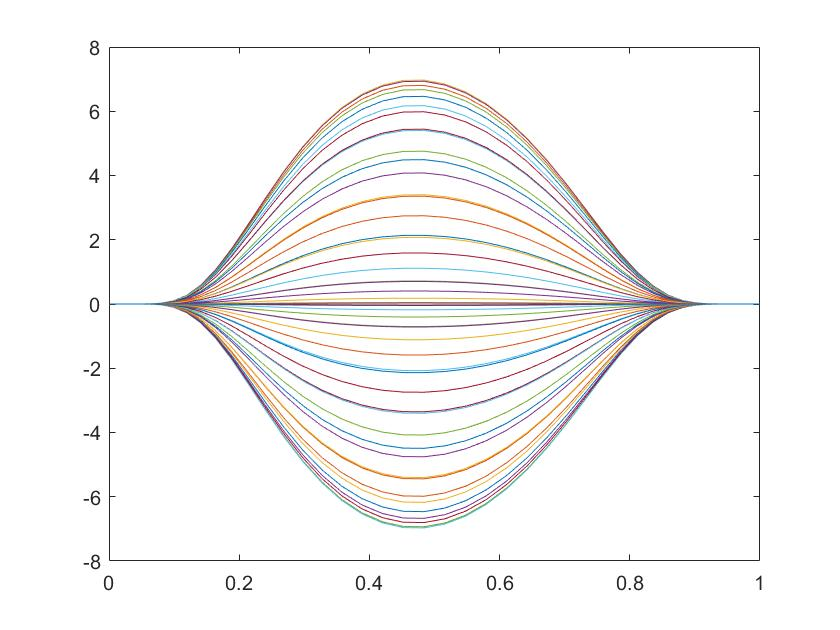
\includegraphics[scale=0.3]{Dexperr1.jpg}
	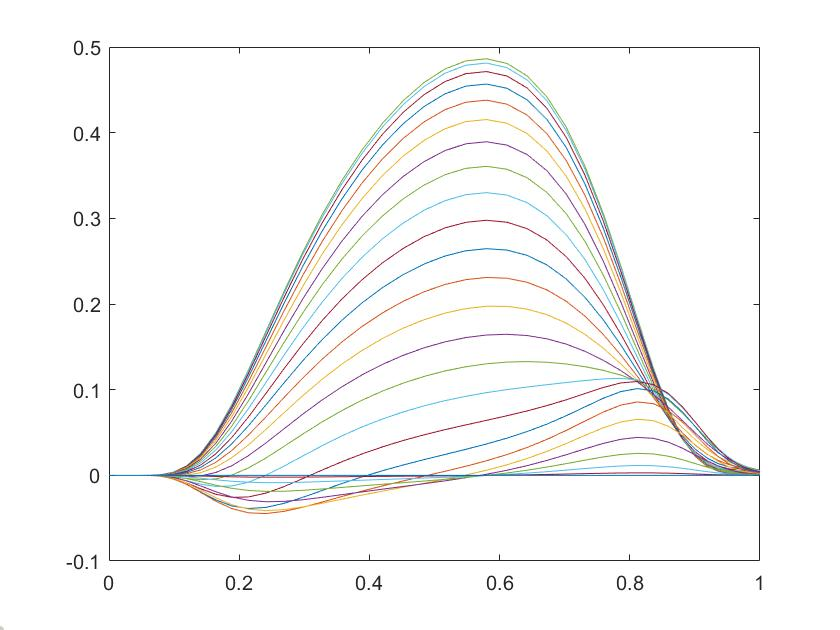
\includegraphics[scale=0.3]{Dexperr2.jpg}
	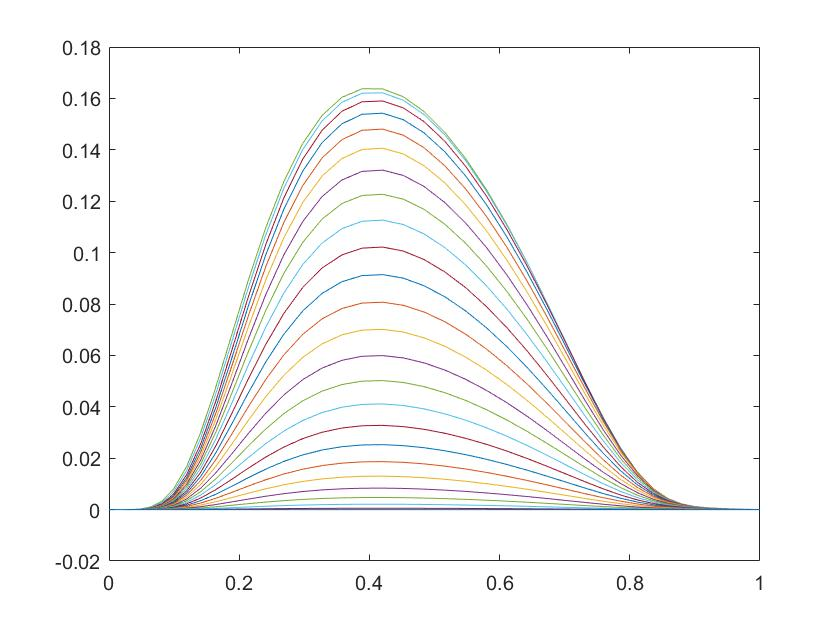
\includegraphics[scale=0.3]{Dexperr3.jpg}
	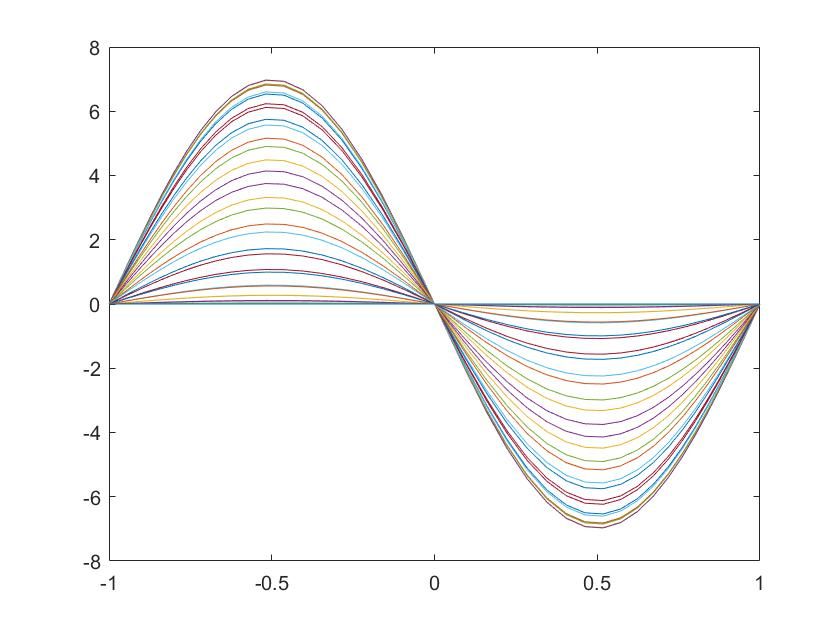
\includegraphics[scale=0.3]{Dexperr4.jpg}
	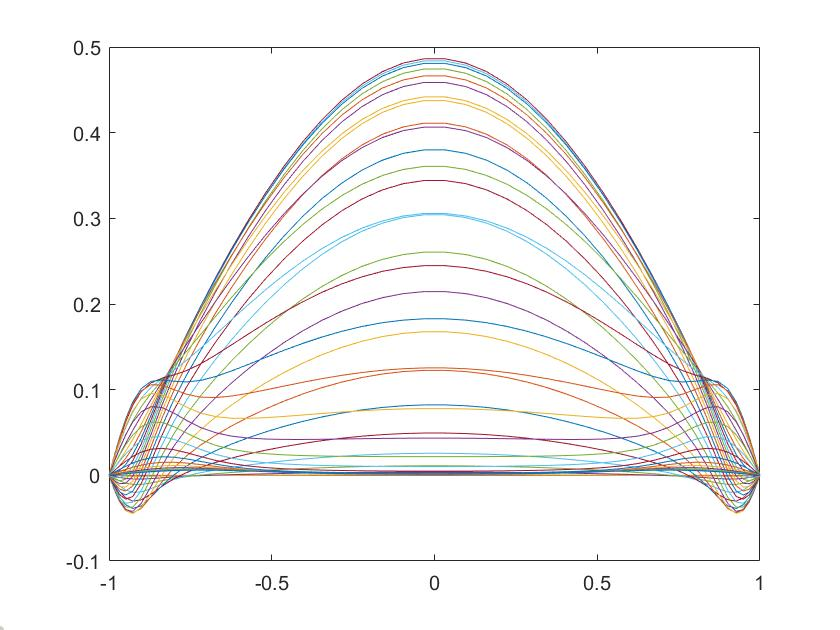
\includegraphics[scale=0.3]{Dexperr5.jpg}
	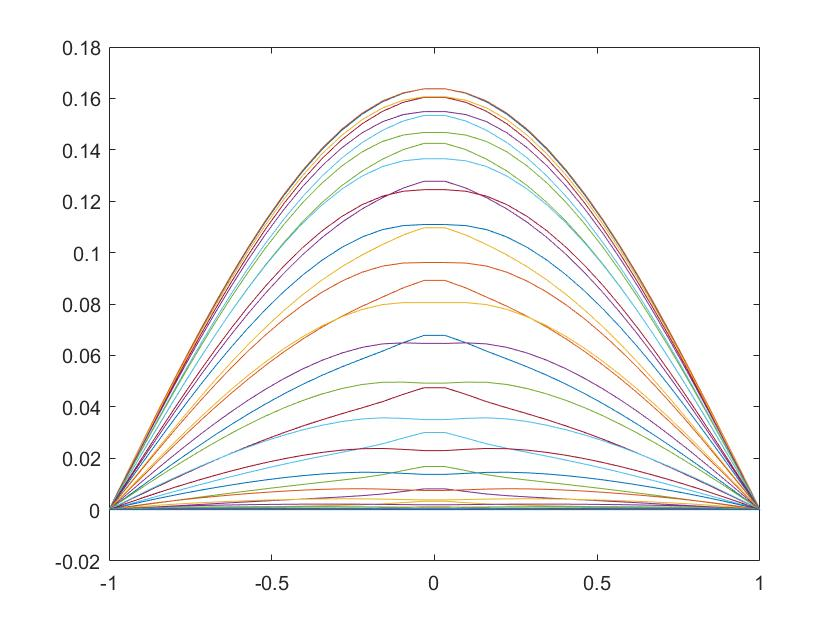
\includegraphics[scale=0.3]{Dexperr6.jpg}
	\caption{Error in $w$, $\rho$, $p$ (first three in time, second three in space) at a perturbation of $0.1 \tilde g(t)$.}
	\label{Dexperr1}
\end{figure}
\begin{figure}[h]
	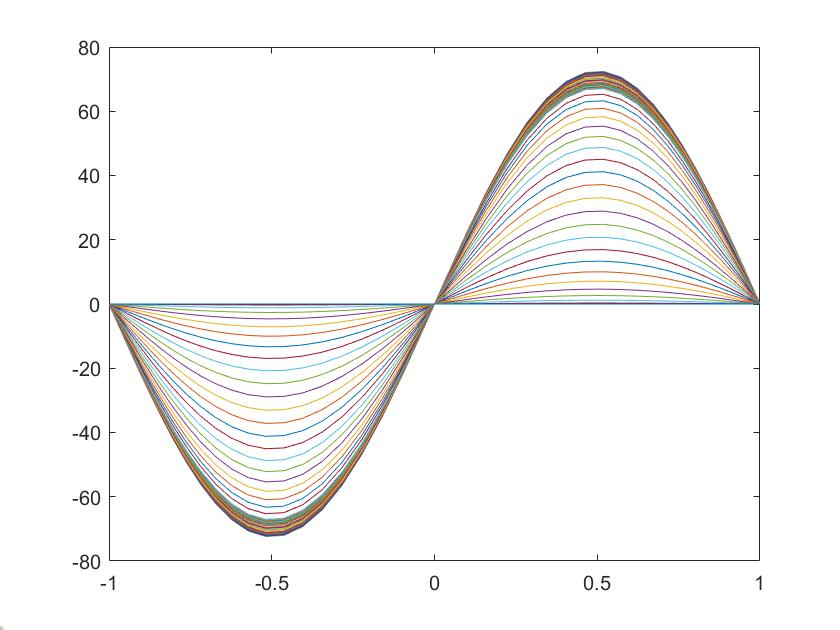
\includegraphics[scale=0.3]{Dexpw1.jpg}
	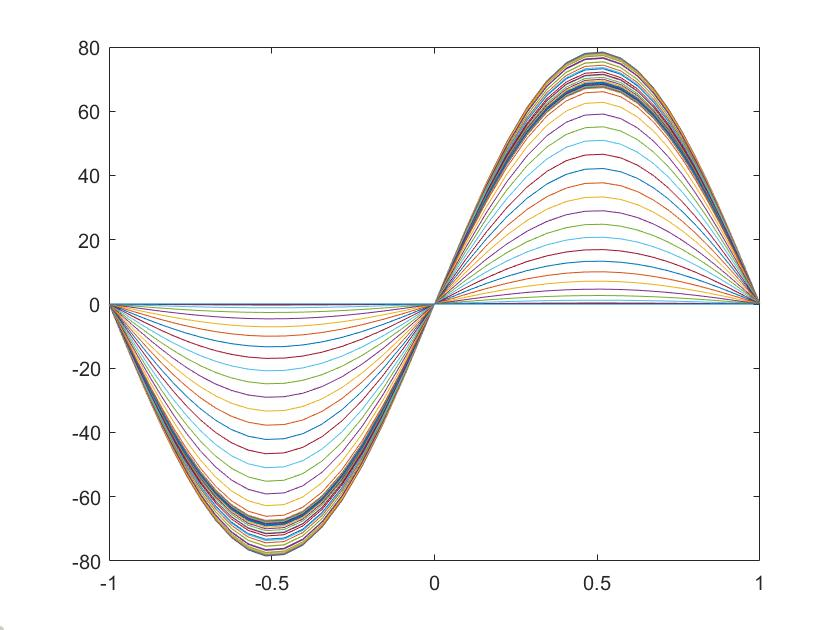
\includegraphics[scale=0.3]{Dexpw2.jpg}
	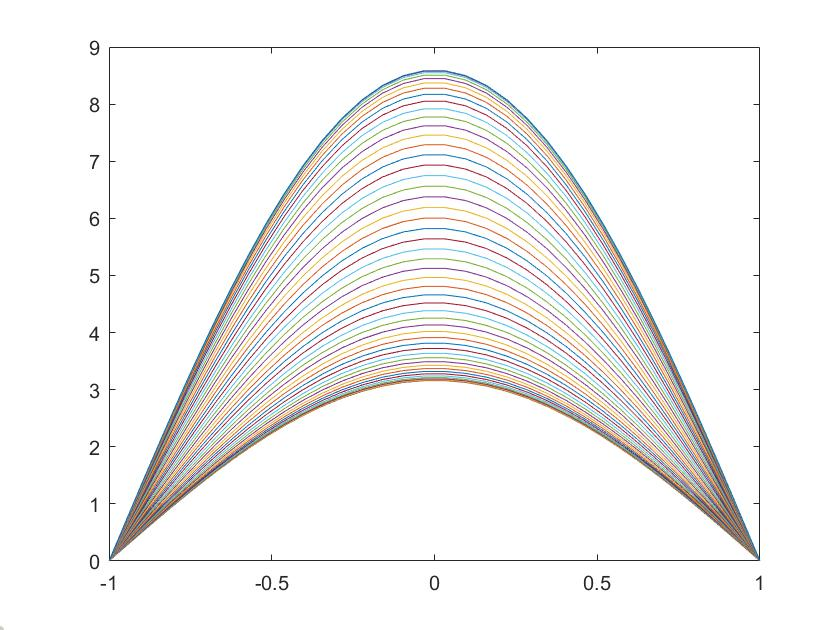
\includegraphics[scale=0.3]{Dexprho1.jpg}
	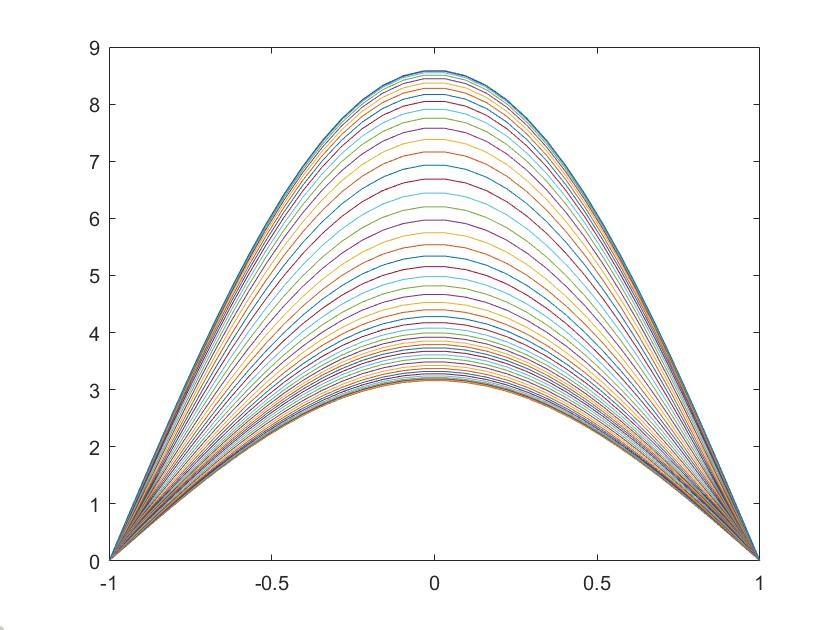
\includegraphics[scale=0.3]{Dexprho2.jpg}
	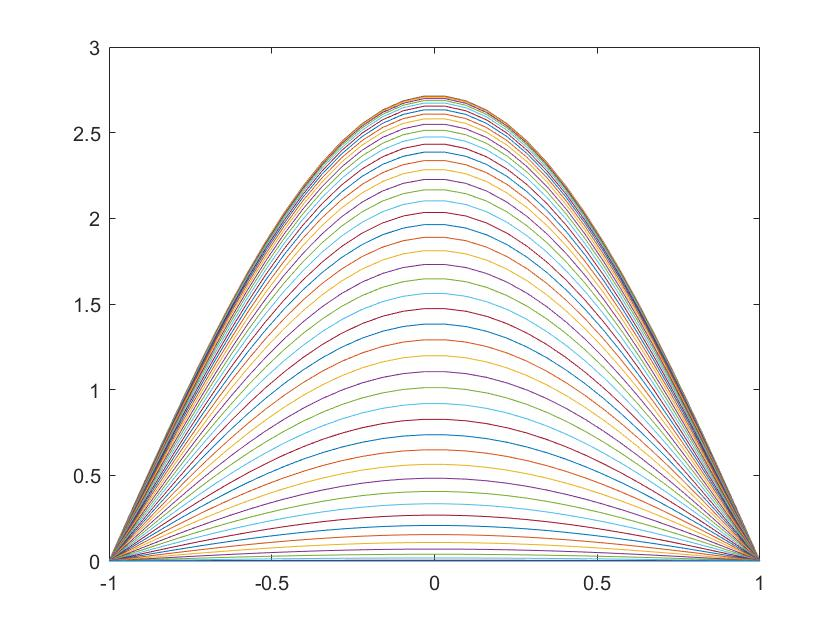
\includegraphics[scale=0.3]{Dexpp1.jpg}
	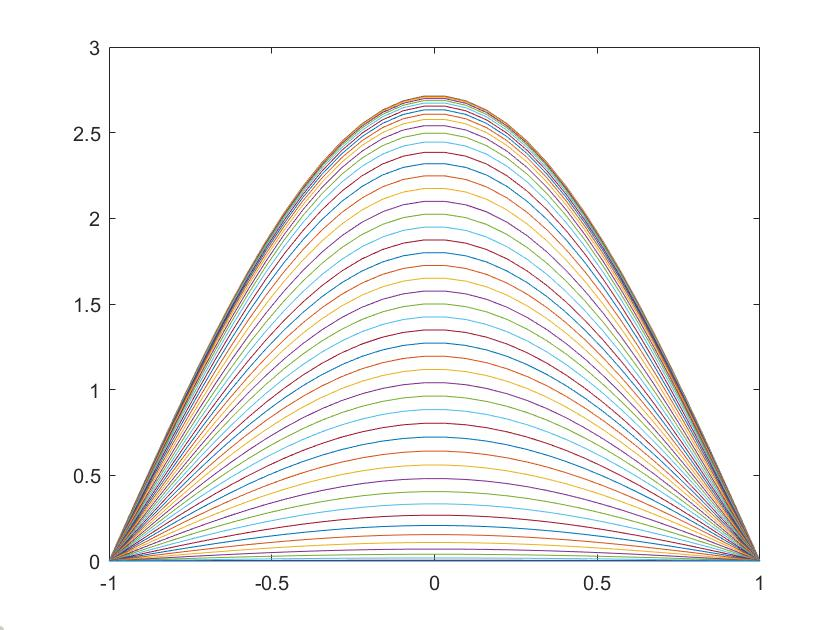
\includegraphics[scale=0.3]{Dexpp2.jpg}
	\caption{$w$, $\rho$, $p$ (first three unperturbed, second three perturbed) at a perturbation of $0.1 \tilde g(t)$.}
	\label{Dexpsol1}
\end{figure}
\subsubsection{Neumann - linear $t$}
Scaled version converges ($w$ max $1$), with $5$ times $\rho$ and $p$ (scaled)($w$ magnitude $25$) diverges at $1.0018 \times 10^{-5}$. In Figure \ref{Nlinrho1} we can compare the unperturbed and perturbed $\rho$ when multiplied by $5$ and the perturbed $\rho$ that is multiplied by $10$. It shows a clear increase in perturbation, so that is probably the reason for the lack of convergence.
\begin{figure}[h]
	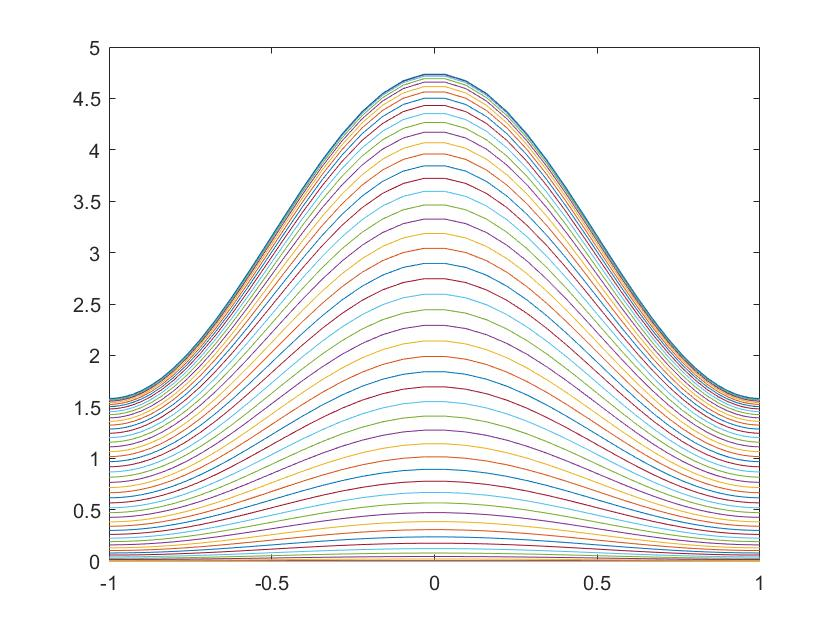
\includegraphics[scale=0.3]{Nlinrho1.jpg}
	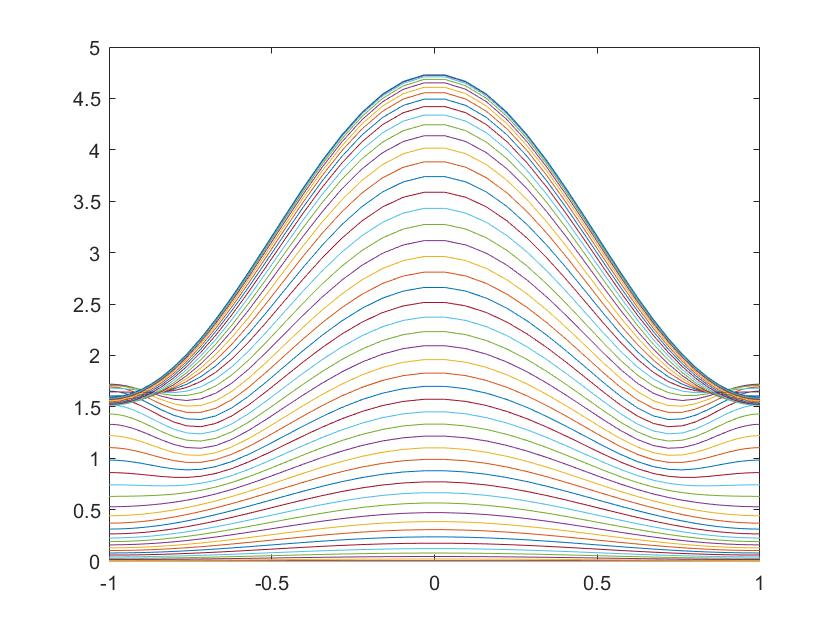
\includegraphics[scale=0.3]{Nlinrho2.jpg}
	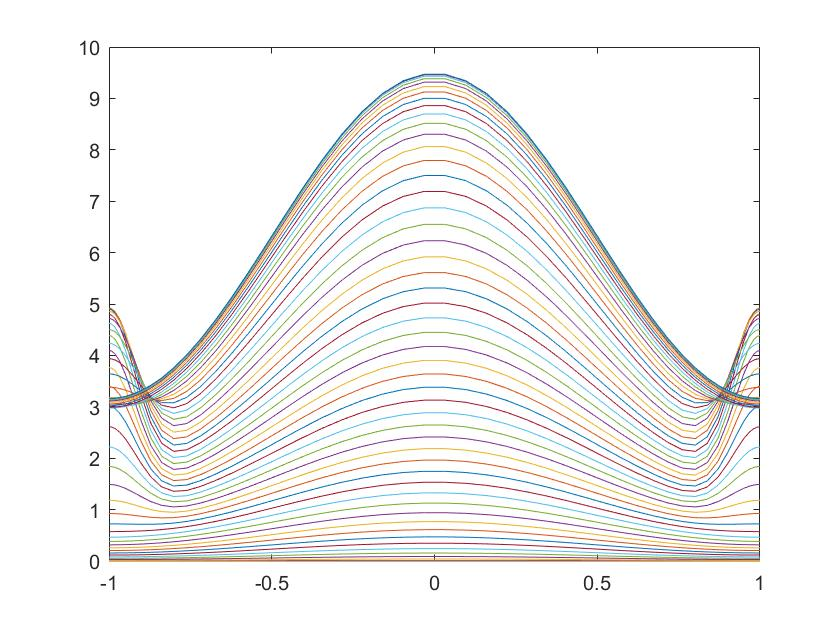
\includegraphics[scale=0.3]{Nlinrho3.jpg}
	\caption{Different magnitudes of $\rho$ have an effect on it's shape; at a perturbation of $0.1 \tilde g(t)$.}
	\label{Nlinrho1}
\end{figure}
\subsubsection{Neumann - exponential $t$}
The unscaled version has $w$ of magnitude $25$ so this doesn't converge ($0.1 \tilde g(t)$), see Figure \ref{Nexperr2}. When choosing $p$ as is and $0.5\rho$, the magnitude of $w$ becomes $13$ and this converges within $896$ Iterations, see Figure \ref{Nexperr1}. 
Looking at how $\rho$ is perturbed, the bigger $\rho$ is, it is not surprising it doesn't converge, see Figure \ref{Nexperr3}. This couldn't be observed in the same way for the Dirichlet case but I think it is probably similar (only not as obvious in Figures \ref{Dexperr1} and \ref{Dexpsol1}). 
\begin{figure}[h]
	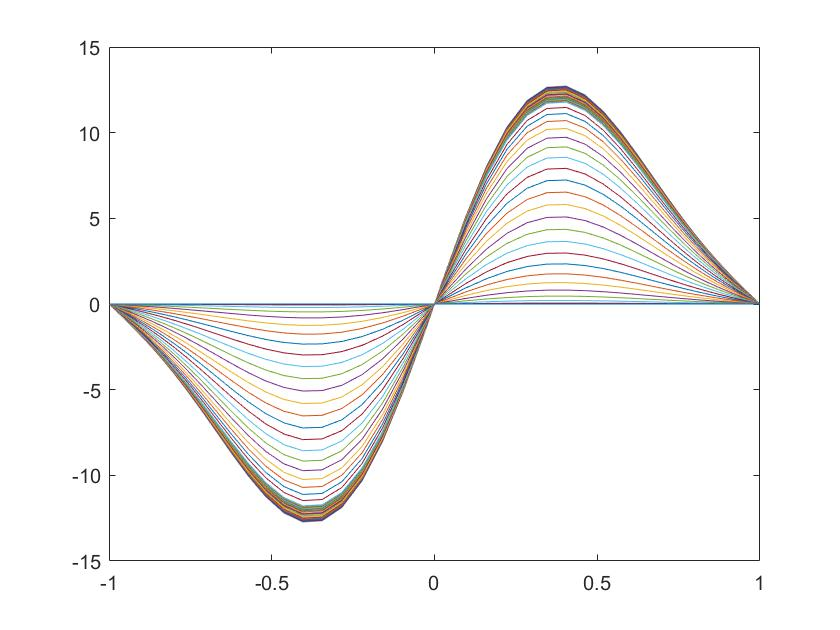
\includegraphics[scale=0.3]{Nexpw1.jpg}
	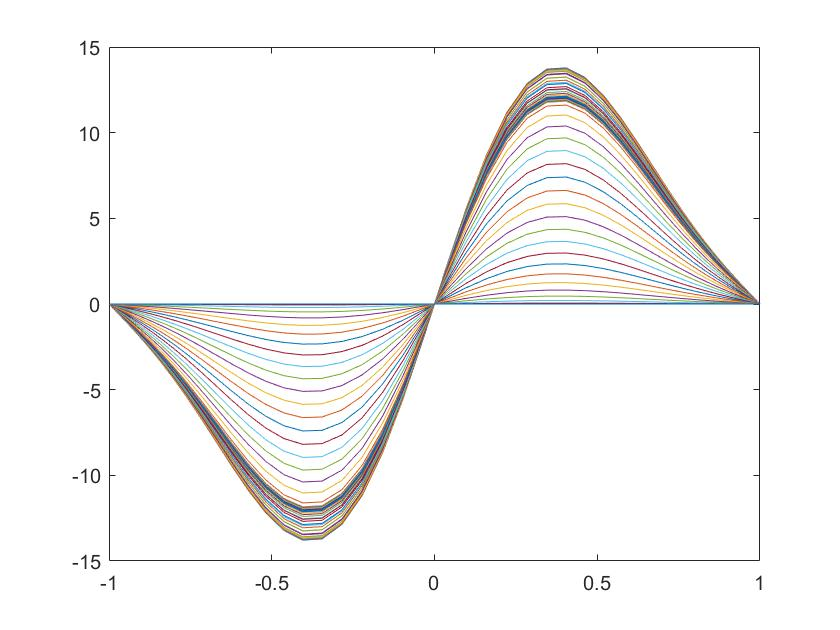
\includegraphics[scale=0.3]{Nexpw2.jpg}
	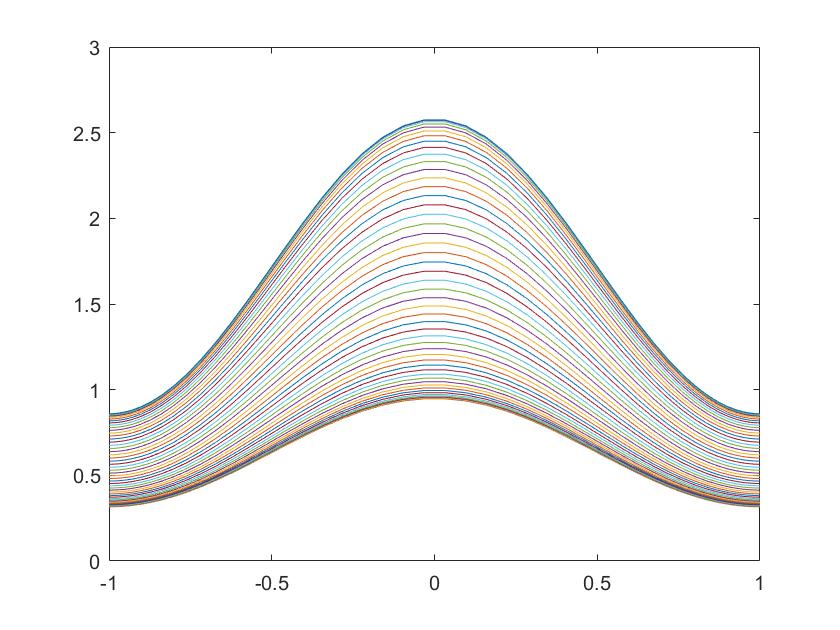
\includegraphics[scale=0.3]{Nexprho1.jpg}
	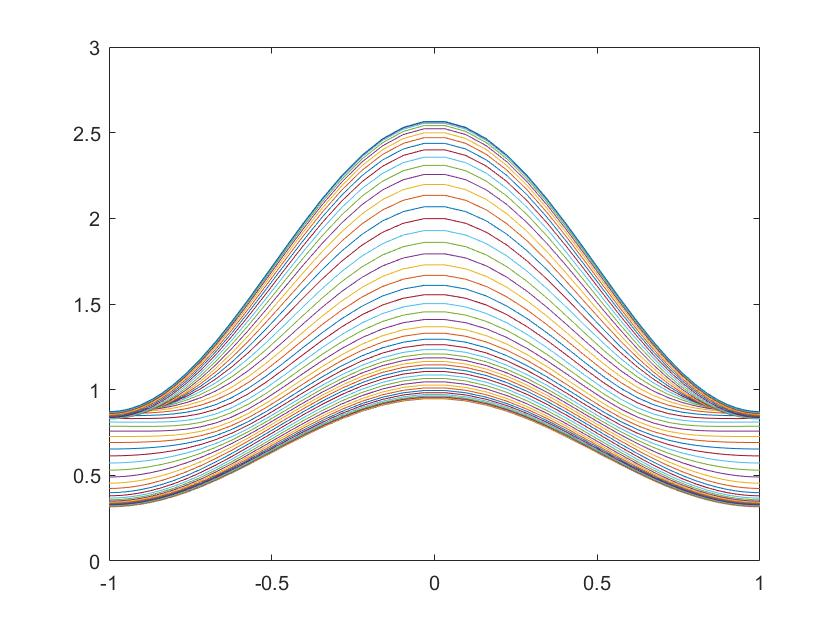
\includegraphics[scale=0.3]{Nexprho2.jpg}
	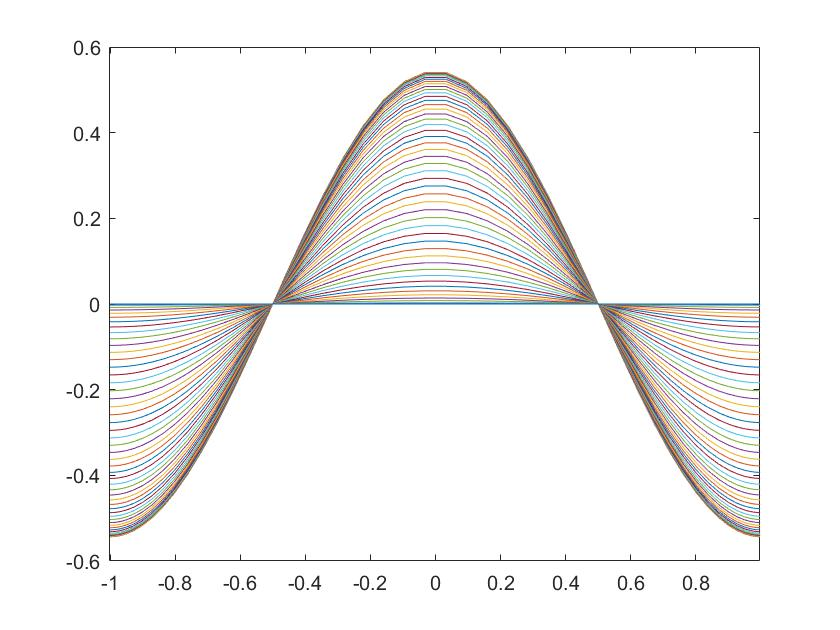
\includegraphics[scale=0.3]{Nexpp1.jpg}
	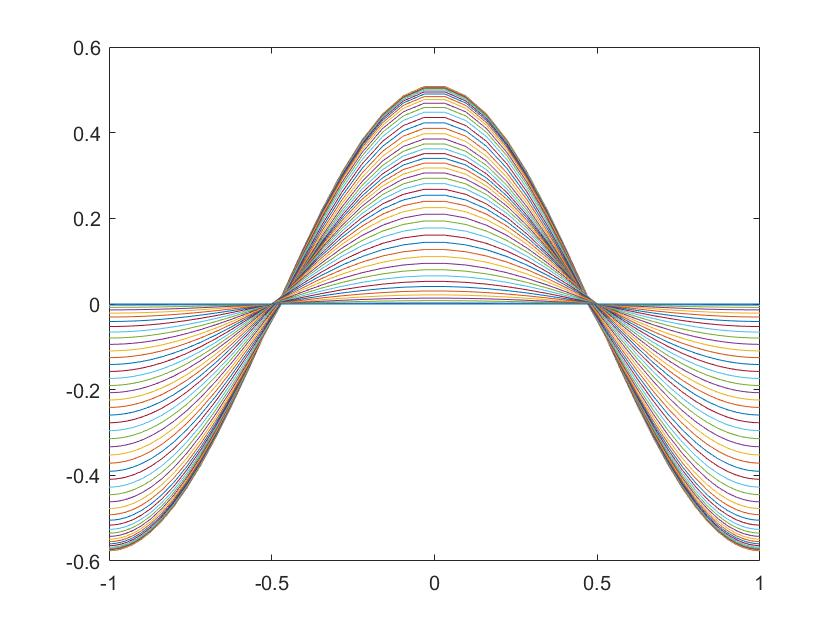
\includegraphics[scale=0.3]{Nexpp2.jpg}
	\caption{$w$, $\rho$, $p$ (exact right, perturbed left) at a perturbation of $0.1 \tilde g(t)$.}
	\label{Nexperr1}
\end{figure}
\begin{figure}[h]
	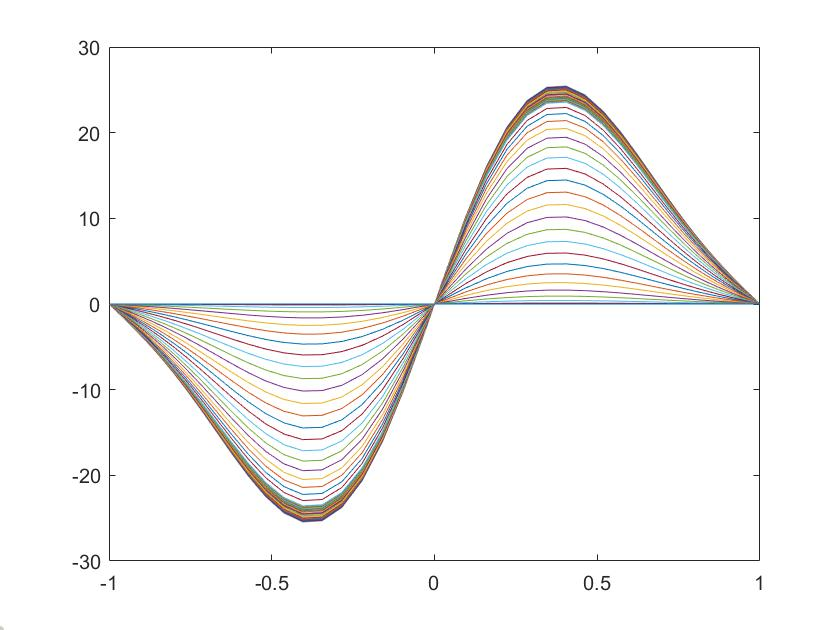
\includegraphics[scale=0.3]{Nexpw1a.jpg}
	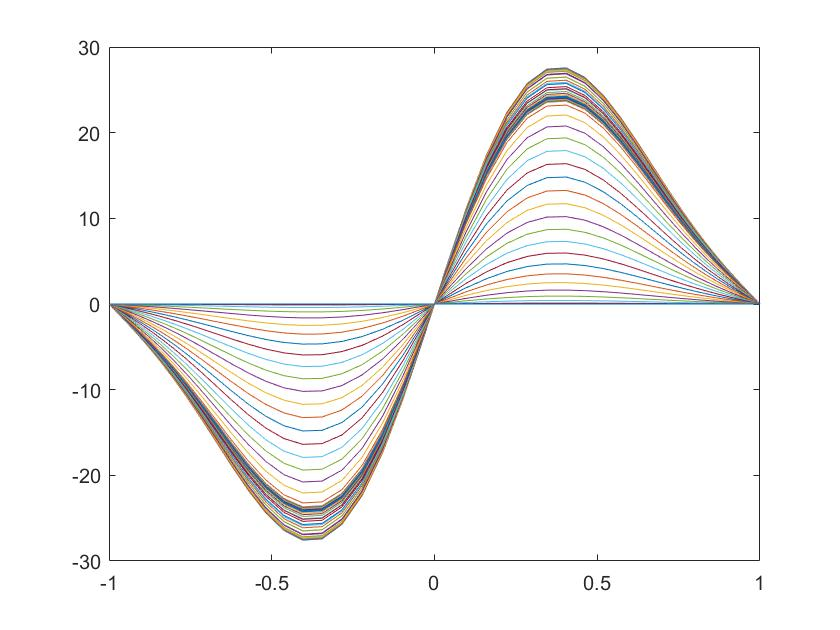
\includegraphics[scale=0.3]{Nexpw2a.jpg}
	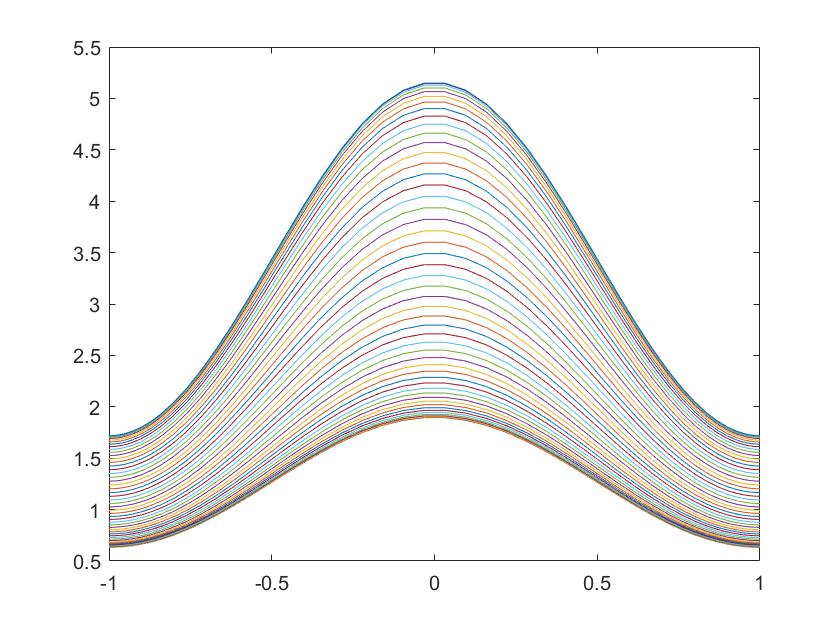
\includegraphics[scale=0.3]{Nexprho1a.jpg}
	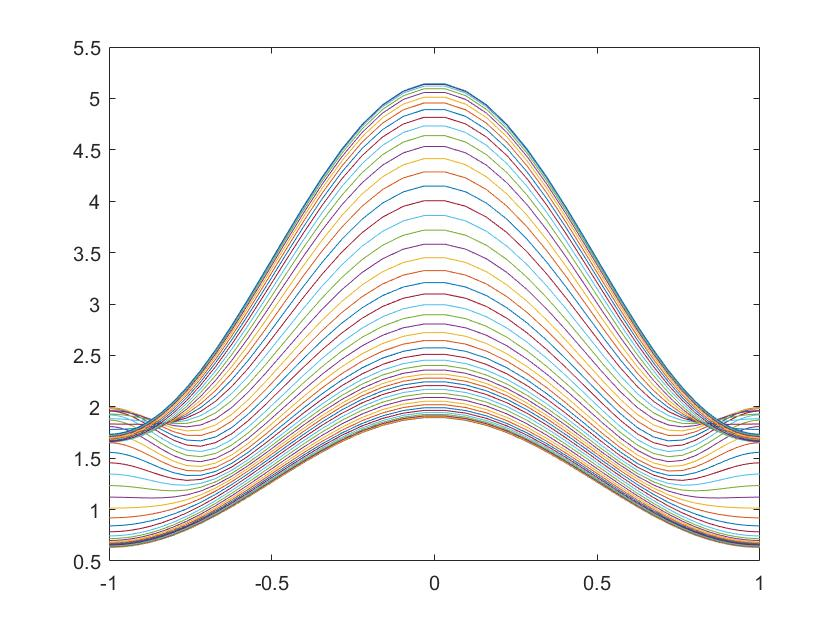
\includegraphics[scale=0.3]{Nexprho2a.jpg}
	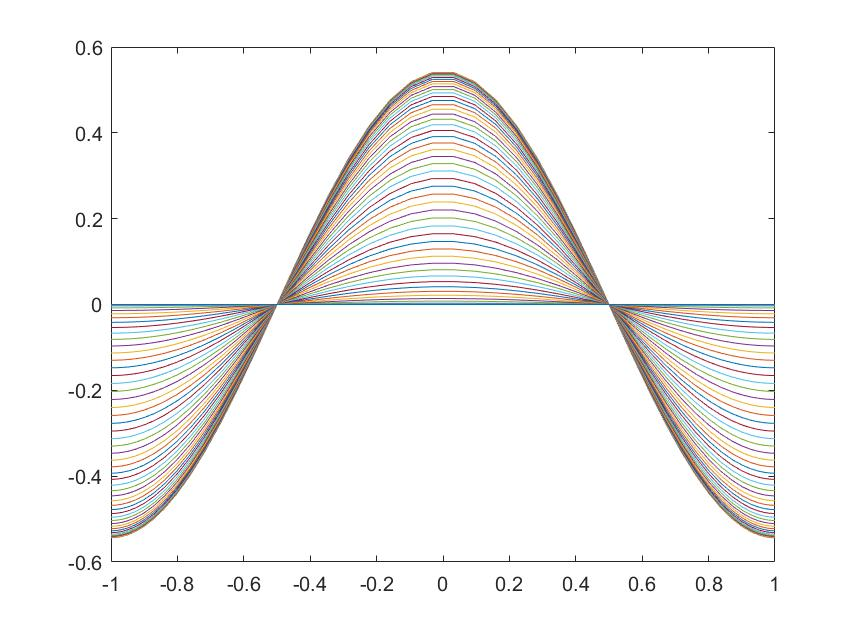
\includegraphics[scale=0.3]{Nexpp1a.jpg}
	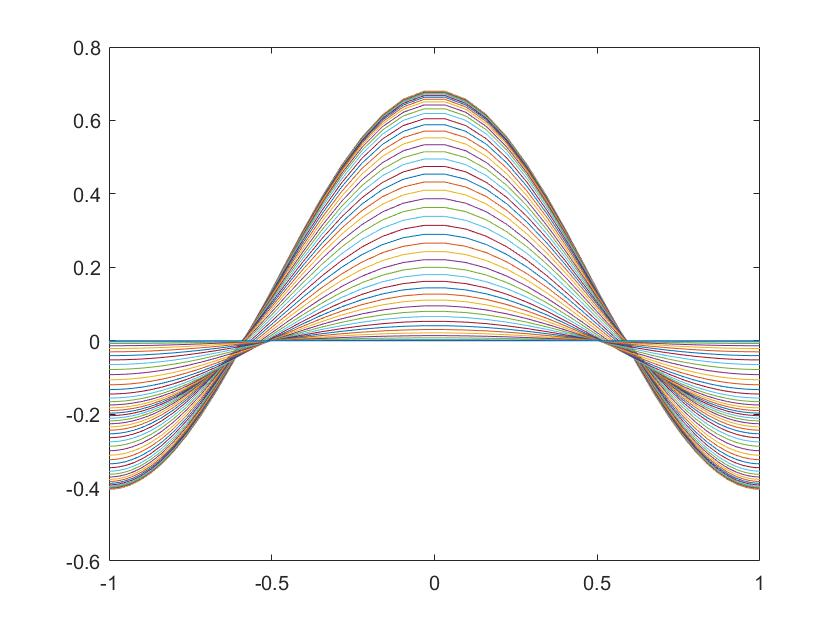
\includegraphics[scale=0.3]{Nexpp2a.jpg}
	\caption{$w$, $\rho$, $p$ (exact right, perturbed left) at a perturbation of $0.1 \tilde g(t)$.}
	\label{Nexperr2}
\end{figure}
\begin{figure}[h]
	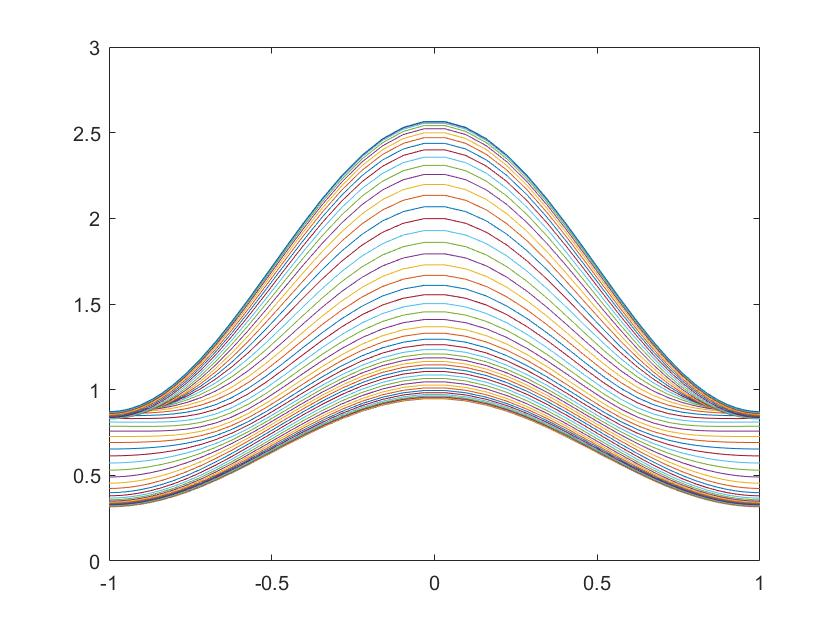
\includegraphics[scale=0.3]{Nexprho2.jpg}
	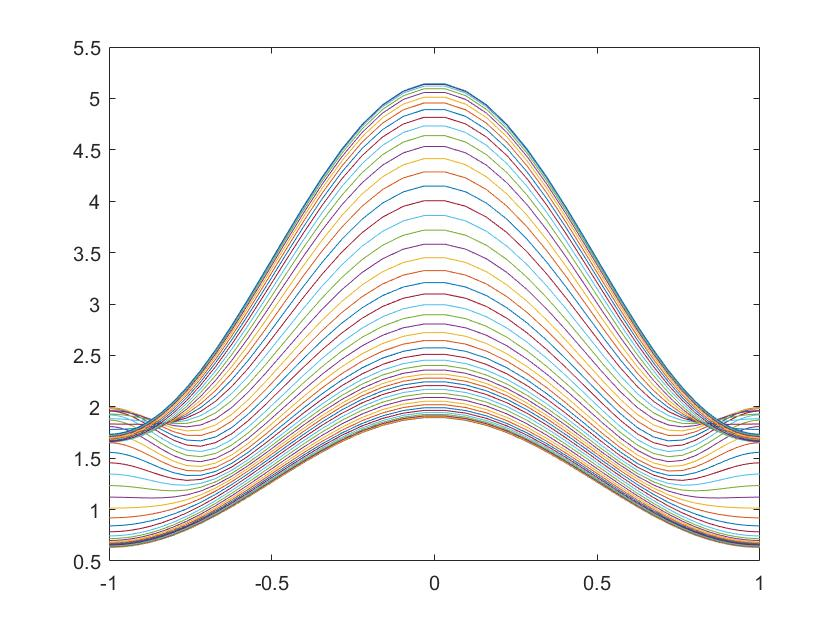
\includegraphics[scale=0.3]{Nexprho2a.jpg}
	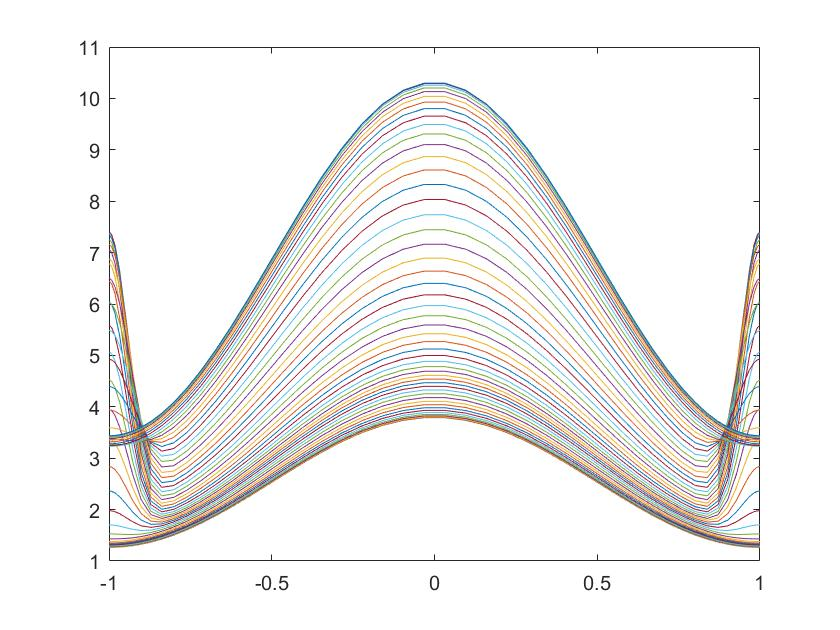
\includegraphics[scale=0.3]{Nexprho2b.jpg}
	\caption{Different magnitudes of $\rho$ have an effect on it's shape; at a perturbation of $0.1 \tilde g(t)$.}
	\label{Nexperr3}
\end{figure}
\subsection{Multiple Shooting}

\subsubsection{Dirichlet - linear $t$}
Choose $N=n=20$.
For $\epsilon = 1$ and $\epsilon =10$ this converges for a range of $\beta$ values. Tried $\epsilon =1$ with $\beta = 10^{-5}$ and $\epsilon=10$ with $\beta =10^3$. Both work without problems. Note, this is a very 'small problem' of max $w = 0.4$.
As in Kalise, the algorithm starts to diverge when $w$ is of order $10$. Here it diverges even a bit before Kalise, at a consistency of $0.00017547$, however $\rho$ and $p$ already diverged before that.
\subsubsection{Dirichlet - exponential $t$}
Choosing $1\rho$ and $2p$, the algorithm converges in $620$ Iterations, from an initial error of $0.05394700$, with $\rho_{errI}= 0.04988878$ and $p_{errI} = 0.0038944$, to the final error of $\rho_{err} = 0.000007217$ and $p_{err} = 0.00005852$. This also converges in Kalise.\\
Next try $1.3 \rho$, $2p$, which just about does not converge in Kalise. As expected, the algorithm diverges, however already at $0.00021012$ (Iteration $428$), which is much earlier than the Kalise algorithm. Furthermore, $\rho$ and $p$ diverge even earlier.

\subsubsection{Neumann - linear $t$}
Try the same example as with Kalise: scaled linear problem - $w$ is of magnitude $1$.
This converges in $482$ Iterations from $0.00405386$, with $\rho_{errI}= 0.00829475$ and $p_{errI}=0.00025015$ to $\rho_{err} = 0.00000026$ and $p_{err}=0.00005884$.
Next try $5 \rho$ and $5p$ to see whether it converges, since Kalise almost does. It diverges at $0.00181230$, which is odd considering Kalise converges down to $1.0018 \times 10^{-5}$..
\subsubsection{Neumann - exponential $t$}
We try $0.5 \rho$ and $1p$, which converges with the Kalise algorithm. The initial error is $0.0201910$, with $\rho_{errI} = 0.01748631$ and $p_{errI}= 0.00124180$. This converges up to $0.00008415$ at Iteration $314$ and then diverges again.\\
Next we try $0.2 \rho$ and $0.8 p$ which definitely converge with Kalise. This converges in $462$ Iterations from $0.00233935$, with $\rho_{errI} = 0.00325195$ and $p_{errI} = 0.00020127$ to $\rho_{err} = 0.00000015$ and $0.00007419$.

\section{Testing $\tilde h(x)$ (briefly)}
Tested linear Dirichlet on two examples, one that does and one that doesn't converge with $0.1\tilde g(t)$. Perturbation $0.1 \tilde h(x)$ has a similar effect. The first example converges as well, the second one diverges at $0(10^{-4})$ which is in agreement with the time perturbation.\\
Tested exponential Neumann case with two examples as well. Here, the example $0.5 \rho$ and $1p$ does not converge, while it converges for the time perturbation, it diverges at $1.5961 \times 10^{-4}$. When choosing $0.25 \rho$ and $1p$ it diverges at $1.0326 \times 10^{-5}$ (almost converges).

\end{document}

\section{Testing $\tilde g(t) \tilde h(x)$ on different exact solutions}
\subsection{Kalise}
\subsubsection{Neumann - linear $t$}
\subsubsection{Neumann - polynomial $t$}
\subsubsection{Neumann - exponential $t$}
\subsubsection{Dirichlet - linear $t$}
\subsubsection{Dirichlet - polynomial $t$}
\subsubsection{Dirichlet - exponential $t$}
\subsection{Multiple Shooting}
\subsubsection{Neumann - linear $t$}
\subsubsection{Neumann - polynomial $t$}
\subsubsection{Neumann - exponential $t$}
\subsubsection{Dirichlet - linear $t$}
\subsubsection{Dirichlet - polynomial $t$}
\subsubsection{Dirichlet - exponential $t$}


